\chapter{An advanced application: situated natural language processing}
\label{chapter|dialogs}

%%%%%%%%%%%%%%%%%%%%%%%%%%%%%%%%%%%%%%

\fxwarning{Mention and detail immanent communication -> context sharing}

\section{Grounding human interaction into the robot knowledge}
\label{sect|dialogs}

\subsection{Situated speech acts}
\label{intro_example}

A messy table, covered with cardboard boxes, books, video tapes... Thomas is
moving and packs everything with the help of Jido, its robot.

`` -- Jido, give me this'', says Thomas, looking at a box that contains a video
tape. The robot smoothly grasps the tape, and hands it to the human.

While this kind of interaction should hopefully sound quite familiar in a
foreseeable future, our robots are not yet quite up to the task. Neither
regarding natural language understanding nor plan-making and manipulation.

To be combined together, those abilities require an unambiguous and shared
representation of concepts (objects, agents, actions...) underlying the
interaction: what are the prerequisites for such a
human sentence --- ``Jido, give me this'' --- to be understood by the robot,
correctly interpreted in the spatial context of the interaction, and ultimately
transformed into an action?

Austin~\cite{Austin1962} would have at first glance analyzed such kind of
sentence as a \emph{speech act}, comprising of \emph{locutionary},
\emph{illocutionary} and possibly \emph{perlocutionary} acts. First, we want to
understand the direct meaning of the sentence (\emph{locutionary act}): we must
acquire the sentence, convert it into a useful syntactic form (quite probably
by mean of speech recognition), and understand the semantics of the sentence,
\ie, What is refered by ``\textit{Jido}''? What is ``\textit{give}''? What is
``\textit{me}''? And ``\textit{this}''?

Working in a situated context, we want furthermore to \emph{resolve} these
semantics atoms, \ie ground them in the sensory-motor space of the robot. For
instance, ``\textit{this}'' is a demonstrative pronoun that refers in this
context to the object the human is focusing on, whatever \textit{focusing}
means: here, Thomas is looking at something, which is a possible cue. But it
could as well point at something or refer to some previously mentioned concept. 

\begin{figure}%[!ht] 
	\centering
	\includegraphics[width=0.9\linewidth]{images/dialogs/pt.jpg} 
	\caption{Interacting with
	the robot in an everyday setup: the human asks for help in vague terms, the
	robot takes into account the human's spatial perspective to refine its
	understanding of the question.} 
	\label{fig|vpt} 
\end{figure}


Second, the \emph{illocutionary force}, \ie the \emph{intent} of the utterance
as thought by the agent must be extracted, and understood. In our example,
Thomas obviously wants an action to be performed by the robot. The action
parametrization is conveyed by the semantics attached to the words and the
grammatical structures of the sentence. In our example, the type of action is
given by the verb ``\textit{give}''. Assuming the robot has some procedural
knowledge attached to this symbol, the action type can be considered as
grounded for the robot. We can as well understand that the recipient of the
action is the human, the performer is the robot itself, and the object acted
upon is the tape. These are the basic \emph{thematic roles}~\cite{Gruber1965}
that can be extracted from the sentence that allow to fully ground the action.

\subsection{Building a symbolic model}

Extracting these speech acts and turning them into a content processable by the
robot is a difficult challenge in the general case. We base our approach on
three distinct, inter-related cognitive functions:

\begin{inparaenum}[\itshape 1)]

\item \emph{Physical environment modeling} and \emph{spatial reasoning}
(grouped under the term \emph{situation
assessment})  are in charge of building and
maintaining a coherent model of the physical world. This model is realistic in
the sense that it relies on accurate 3D models of both manipulated objects and
humans. It also has dedicated mechanisms to manage disappearing or occluded
objects.  The geometric model is used to compute several spatial properties of
the scene that actually convert the original sensory data into symbolic
beliefs. This includes relative locations of objects, visibility state,
gestures like pointing, etc.  Assuming that other agents are as well
represented in the model, the same computations are applied to analyze the
scene from each agents' point of view (\ie from their \emph{perspectives}).
This approach is presented in depth in~\cite{Sisbot2011}.

\item \emph{Knowledge representation and management}: the robot is endowed with
an active knowledge base that provides a logically sound symbolic model of its
beliefs on the world, as well as models for each cognitive agent the robot
interacts with. Each of these models is independent and logically consistent.
This enable reasoning on different perspectives of the world that would be
considered otherwise inconsistent (for instance, an object can be visible for
the robot but not for the human. This object can have at the same time the
property {\tt isVisible \textbf{true}} and {\tt isVisible \textbf{false}}, in
two different models).  Our platform also features continuous storage, querying
and event triggering over the pool of facts known by the robot. It relies on
OWL ontologies (a decidable subset of the predicate logics). The knowledge base
is presented in~\cite{Lemaignan2010}.

Used in combination with the situation assessment framework, the robot is thus
able to maintain different models of the world, one per agent. This proves an
essential feature (\cite{Roy2005, Kruijff2010}) to enable perspective-aware
grounding of natural language, as we will see in next sections.

\item \emph{Dialogue input processing}, including natural language parsing
capabilities, disambiguation routines and interactive concept anchoring. We
focused our efforts on three classes of utterance, commonly found in
human-robot interaction: \emph{statements} (\ie new facts the human wants to
inform the robot), \emph{orders} (or more generically \emph{desires}) and
\emph{questions on declarative knowledge} (whose answers do not require
explicit planning). This would roughly cover the \emph{representative}
(sometimes referred as \emph{assertives}) and \emph{directives} type of
illocutionary acts, in Searle~\cite{Searle1976} classification. This paper
focuses on this last facet (dialogue processing).

\end{inparaenum}

\subsection{Related work}

Processing natural language in situated context is already an established
research field. In~\cite{Roy2005}, Roy summarizes what he sees as the main
challenges to be tackled: cross-modal representation systems, association of
words with perceptual and action categories, modeling of context, figuring out
the right granularity of models, integrating temporal modeling and planning,
the ability to match past (learned) experiences with the current interaction
and the ability to take into account the human perspective.

Kruijff et al. provides in~\cite{Kruijff2010} an up-to-date survey of literature
on situated human-robot dialogue, focusing on formal representation systems,
bi-directionality of the interaction and context building. They point as well
that, compared to the cognitive psychology community, the ``situated AI''
community started only recently to take into account agents focus, perspective and temporal
projection abilities.

Dialogue processing on real robots have been explored by several teams.
Scheutz~\cite{Brick2007} has contributions regarding natural language
processing in an incremental way, and how this enables instant back-channel
feedback (like nodding).

Hüwel et al.~\cite{Huwel2006} propose the concept of \textit{Situated Semantic
Unit}: these meaning atoms are extracted from sentences and expose semantic
links to other units. The parser tries to satisfy these links and rate
accordingly the semantic interpretation of the sentence. Used in conjunction
with ontologies, their approach offers good robustness to ungrammatical or
partial utterances. They validated the approach with an extensive user-study.

While mostly implemented on virtual agents, the GLAIR cognitive architecture
by Shapiro et al.~\cite{Shapiro2009} is an architecture
explicitly built to tackle the grounding issue from the percept to the
decision. The knowledge layer relies on a custom knowledge representation
language, it has natural language processing capabilities similar to ours. It
features explicit management of contexts of facts and memory models (long
term/short term, episodic/semantic).

Also worth mentioning, Mavridis and Roy~\cite{Mavridis2005} propose the idea of
a \emph{grounded situation model} which is an amodal model of the world where
different sensing modalities, including verbal ones (the robot is able to
\emph{imagine} objects), are merged. Their framework also allows management of
the interaction history (the human can ask for a past event). They propose an
implementation in an environment built on simple entities (a manipulator arm
and color balls).

\subsection{Contribution}

Compared to previous contributions, our efforts have two foci: {\it (1)}
integration between language processing and perception of the environment and
the humans, from several perspectives; and {\it (2)} realistic human-robot interactions:
realtime processing; open speech; complex, dynamic, partially unknown human environments; fully
embodied autonomous robots with manipulation abilities. 

We do not claim any contribution to the field of computational linguists (see
\cite{Kruijff2010} for a survey of formal approaches to natural language
processing in the robotics field): our main contribution here is the grounding
of concepts involved in the human discourse through the robot's own knowledge.

Section~\ref{dialog} presents the overall grounding process, section~\ref{examples} 
proposes an analysis of the processing of three prototypical sentences. 
Experimental results are presented in section~\ref{experiment}. A 
discussion regarding the current limitations of our system concludes
this article.

%%%%%%%%%%%%%%%%%%%%%%%%%%%%%%%%%%%%%
\section{The Natural Language Grounding Process}
\label{dialog}

Verbal interaction with human presents two categories of challenges: syntactic
ones, and semantic ones. The robot must be able to process and analyze the
structure of human utterances, \ie natural language sentences, and then make
sense of them. As stated in the introduction, we process three categories of
sentences: \emph{statements}, \emph{desires} and \emph{questions} that can be
answered from the declarative knowledge present in the robot knowledge base (a
choice similar to the \emph{Behaviour Cycle} in the GLAIR
architecture~\cite{Shapiro2009}). In our work, the grounding process of the
human discourse consists in extracting either the \emph{informational} content
of the sentence to produce statements or its \emph{intentional} content (\ie
performative value) to collect orders and questions. We do not claim any
contribution to the field of computational linguists (see \cite{Kruijff2010}
for a survey of formal approaches to natural language processing in the
robotics field). Our main contribution here is the grounding (we call it
\emph{resolution}) of concepts involved in the human discourse through the
robot's own knowledge.

We have developed a dedicated module called {\sc
Dialogs}\footnote{\textsc{Dialogs} is an open-source project. Source code is
available from \url{http://dialogs.openrobots.org}.} that processes human
input in natural language, grounds the concepts in the robot's knowledge and
eventually translates the discourse in a set of declarative OWL/RDF statements.

\begin{figure}[!ht]
\centering
  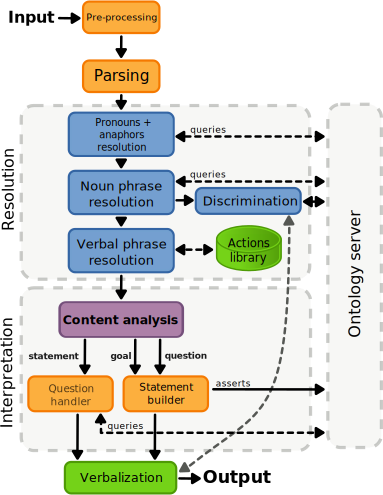
\includegraphics[width=0.6\linewidth]{images/dialogs/dialog_module_simple.pdf}
  \caption{The {\sc Dialogs} module has three main steps: the parsing,
  the interpretation and the verbalization. The interpretation module is
  responsible for both the \emph{resolution} and the semantic content
  \emph{analysis and translation}.} 
  \label{fig|dialog}
\end{figure}

As shown in Figure~\ref{fig|dialog}, the {\sc Dialogs} module is composed of
three main blocks. The user's input is first pre-processed. For instance,
\emph{I'm} constructs are expanded into \emph{I am} and then parsed. The parser
is a custom-made, rule-based (\ie grammar-free) tool that extracts the
grammatical structure from the user's sentence.

Figure~\ref{dialog|parser_output} shows an example of the raw output of the
parser for a moderately complex sentence.

\begin{figure}%[!ht]
\begin{center}
\scriptsize
\begin{alltt}
>> IMPERATIVE
VP: \textbf{remember} (present simple)
    SUBSENTENCE (aim: that)
      NP: \textbf{I}
      VP: \textbf{want} (present simple)
        direct objects: 
          NP: \textbf{you}
        secondary VP: \textbf{give} ()
              direct objects:
                NP: my \emph{nice blue} \textbf{bottle}
              indirect objects:
                NP: \textbf{me}
\end{alltt}
\end{center}
\caption{Raw output of the {\sc Dialogs} parser after processing the
sentence: ``remember that I want you to give me my nice blue bottle.'' 
Nominal groups are not grounded yet.} 
\label{dialog|parser_output}
\end{figure}

The result of the parsing is then sent to the \emph{interpretation} module, the
core of the approach.  Interpretation consists in three distinct operations:
the sentence \emph{resolution} (concepts grounding), the \emph{content
analysis} (what is the intent of the utterance: information, question or
desire) and the \emph{statement building} (translation into RDF statements).

The sentence resolution has three steps: {\it(1)} pronouns and anaphora are
replaced by, respectively, the correct speaker ID and the ID of the last object
spoken about (extracted from the dialogue history), {\it(2)} nominal groups are
disambiguated and grounded (noun phrase resolution), and {\it(3)} verbal groups
are resolved as well, and their associated thematic roles are retrieved (verbal
phrase resolution). Algorithm~\ref{algo|Resolution} describes the overall
process.  Next section describes specific examples to show how the noun and
verbal phrase resolution takes place.

\small
\begin{pseudocode}[ruled]{Resolution}{sentence, currentSpeaker}
\label{algo|Resolution}

\mathcal{G} \GETS \CALL{ParseNominalGroups}{sentence} \\

\FOREACH g \in \mathcal{G} \DO 
\BEGIN
   \mathcal{D} \GETS \CALL{GenerateDescription}{g} \STMTNUM{5.1em}{res.desc}\\
   candidates \GETS \CALL{Ontology.Find}{\mathcal{D}} \STMTNUM{4em}{res.onto}\\
   
   \IF \left|{candidates}\right| = 0 \THEN
    \BEGIN
      \OUTPUT{\mbox{Couldn't resolve the group!}} \\
      \EXIT \\
    \END
   \ELSEIF \left|{candidates}\right| = 1 \THEN
      id \GETS candidates[0] \STMTNUM{8em}{res.easy}\\

   \ELSE
      \BEGIN
	\IF \CALL{Ontology.CheckEquivalent}{candidates} \THEN
	  id \GETS candidates[0] \\
	\ELSE
	  id \GETS \CALL{Discrimination}{candidates} \\ %\STMTNUM{1em}{st.discrimination}\\
      \END \\
   \CALL{Replace}{g, id, sentence}
\END
\end{pseudocode}
\normalsize

As represented in Figure~\ref{fig|dialog}, interpretation tightly relies on the
communication with the knowledge base. All the concepts the robot manipulates
are stored in the ontology server and retrieved through logical
queries, except for the verbs that are currently stored in a dedicated library
(the \emph{action library} in the diagram).

%%%%%%%%%%%%%%%%%%%%%%%%%%%%%%%%%%%%%
\section{Technical analysis}
\label{examples}

In order to better understand the overall process of the {\sc Dialogs} module
and its relation with ORO, we next describe the different steps of the approach
based on three examples. In these examples we assume that some initial facts
are present in the knowledge base (section~\ref{modeling_real_world} discusses
how the initial knowledge can be acquired), both in the robot's own model and
in the human's model.  Since the robot tries to ground a human utterance, all
queries are sent to the human model in order to interpret it from the human
perspective.

\subsection{Informational Content Extraction}
\label{informational_content_extraction}

\begin{figure}
    \centering
%	\begin{tabular}{p{0.5\columnwidth} | p{0.5\columnwidth}}}
	\begin{tabular}{l|l}
	\emph{Initial knowledge} \texttt{human\_01} &
	\emph{Human input}\\	
	
	\hline

    	\stmt{banana\_01 type Banana} &
	``The yellow banana is big!'' \\
	
    	\stmt{banana\_01 hasColor yellow} & \\
	\vspace{0.5em}\\
	\hline

	\emph{Generated partial statements} &
	\emph{Newly created statements}\\
	\hline

	\stmt{?obj type Banana} &
	\hspace{0.2cm}\stmt{banana\_01 hasSize big} \\
	
    	\stmt{?obj hasColor yellow} & \\
    	\hspace{0.2cm}$\Rightarrow$ \concept{?obj = banana\_01}\\

	\hline
	\end{tabular}
\caption{First example: content extraction.
``$\Rightarrow$'' represents the output of the ontology server.}
\label{dialog|ex1}
\end{figure}


Figure~\ref{dialog|ex1} shows a first example of human discourse grounding and
the extraction of informational content. We assume that the robot knowledge
base only contains two initial statements in the human model. The user asserts
a new one: ``The yellow banana is big!''.  We first want to match the nominal
group \emph{The yellow banana} to an already known concept
(algorithm~\ref{algo|Resolution}), and second to translate the property
\emph{is big} into a predicate ({\tt hasSize}) to state its semantics.


\small
\begin{pseudocode}[ruled]{GenerateDescription}{group}
\label{algo|GenerateDescription}

\PROCEDURE{GenerateDescription}{group} 
   noun \GETS \CALL{GetNoun}{group} \\ 
   \IF \CALL{Ontology.Lookup}{noun} \in (Instances) \STMTNUM{7.5em}{st.lookup} \THEN
   		\BEGIN
		id \GETS \CALL{Ontology.lookup}{noun}\\	
		\RETURN {\mathcal{D} + \{ *\ {\tt sameAs}\ <id> \}}\\
		\END
   \ELSE
    	\mathcal{D} = \mathcal{D} + \{ *\ {\tt type}\ <noun>\} \\
   
   \\
   det \GETS \CALL{GetDeterminant}{group} \\
   \IF det \in {\mbox(possessives)} \THEN
       \mathcal{D} = \mathcal{D} + \{ *\ {\tt isRelatedTo}\ <possessor>\} \\
    
    \IF det \in {\mbox(demonstratives)} \THEN
        \BEGIN
        \IF \CALL{Ontology.Check}{\{<currentSpeaker>\ {\tt focusesOn}\ *\}} \THEN 
            \mathcal{D} = \mathcal{D} + \{<currentSpeaker>\ {\tt focusesOn}\ *\}
        \ELSE
            \mathcal{D} = \mathcal{D} + \CALL{AnaphoricMatching}{} \STMTNUM{4em}{st.anaphoric} \\
        \END \\
   \\
   adjs \GETS \CALL{GetAdjectives}{group} \\
   \FOREACH adj \in adjs \DO
   	\BEGIN
   		\IF adj == <other> \THEN 
   			\BEGIN
   			id \GETS \CALL{History.GetMatchingGroup}{group} \STMTNUM{8em}{st.history}\\
   			\mathcal{D} = \mathcal{D} + \{ *\ {\tt differentFrom}\ <id> \}\\
   			\RETURN{D}\\
			\END   		
   		\ELSE
	     	\mathcal{D} = \mathcal{D} + \{ *\ {\tt hasFeature}\ <adj>\} \STMTNUM{9em}{st.adj} \\
    \END\\
    
   \\  
   nounComplements \GETS \CALL{GetNounComplements}{group} \\
   \FOREACH nouncmpl \in nounComplements \DO
     \mathcal{D} = \mathcal{D} + {\CALL{GenerateDescription}{nouncmpl}}\\
   
   
   \\  
   relativeClauses \GETS \CALL{GetSubordinateRelativeClauses}{group} \\
   \FOREACH relative \in relativeClauses \DO
   	\BEGIN
   	 \mathcal{G} \GETS \CALL{GetNominalGroups}{relative} \\
   	 \FOREACH g \in \mathcal{G} \DO
     	\mathcal{D} = \mathcal{D} + {\CALL{GenerateDescription}{g}}
    \END\\
     
   \\
   \RETURN{\mathcal{D}} 
\ENDPROCEDURE
\end{pseudocode}
\normalsize

\small
\begin{pseudocode}[ruled]{History.GetMatchingGroup}{group}
\label{algo|History}
\PROCEDURE{History.GetMatchingGroup}{group}
\COMMENT{Extract Nominal group from sentences stored in the history}\\
\mathcal{H} \GETS \CALL{History.GetAllNominalGoup}{}\\
\COMMENT{Generate description of the nominal group that is being processed.} \\
\COMMENT{The adjective  "other" is to be removed before calling this routine} \\
	\mathcal{G} \GETS \CALL{GenerateDescription}{group} \\ 
	
	candidates \GETS \mathcal{H} \cap \mathcal{G}\\
	\IF \left|{candidates}\right| = 0 \THEN
    \BEGIN
      \OUTPUT{\mbox{Couldn't find another object with the same characteristics!}} \\
      \EXIT \\
    \END
   \ELSEIF \left|{candidates}\right| = 1 \THEN
      id \GETS candidates[0]
   \ELSE
   	  id \GETS \CALL{Discrimination}{candidates}\\
   \RETURN{id}
\ENDPROCEDURE
\end{pseudocode}
\normalsize

To resolve the nominal group \emph{The yellow banana} a set of partial
statements that describe the concept is generated based on the grammatical
parsing of the sentence (algorithm~\ref{algo|Resolution}(\ref{res.desc})). The
parsed tree of each nominal group is translated into statements based on a set
of rules.  In the example, a banana (\stmt{?obj type Banana}) that is yellow
(\stmt{?obj hasColor yellow})\footnote{Predicates like \concept{hasColor} or
\concept{hasSize} that bind \concept{banana\_01} to adjectives are extracted
from a predefined database of $[Predicate \rightarrow AdjectiveCategory]$, and
falls back on the generic \concept{hasFeature} predicate if the adjective is
not known.}.  Based on these partial statements a SPARQL query is sent to the
ontology server to retrieve possible instances that match the description
(algorithm~\ref{algo|Resolution}(\ref{res.onto})).

In this first simple case, the concept \concept{banana\_01} is unambiguously
matched (since there is only one possible banana) and returned. Finally, we can
now add the new information provided by the human, \ie the new statement
\stmt{banana\_01 hasSize big}, to the human model in the ontology server.

The translation of \emph{yellow} to \stmt{hasColor yellow} is not obvious: in
the general case, we associate a adjective to the noun it characterizes with
the \concept{hasFeature} predicate (for instance, \emph{The sight is beautiful}
would translate to \stmt{sight hasFeature beautiful}). But we can also manually
set the predicate associated to a category of adjectives: It is what has been
done for the main colours. Another example is the size: for known size
adjectives (big, small, etc.), the \concept{hasSize} predicate is being used.


\subsection{Intentional Content Through Verb Resolution}

The sentence in the first example is built with the state verb \emph{be} at
indicative. Let us examine a different example with an action verb at
imperative mode (an order): ``Give me the banana". The process is described in
Figure~\ref{dialog|ex2}.

\begin{figure}
    \centering
	\begin{tabular}{l|l}
	\emph{Initial knowledge} \texttt{human\_01} &
	\emph{Human input}\\
	
	\hline
	
    	\stmt{banana\_01 type Banana} &
	``Give me the banana.'' \\
	
    	\stmt{banana\_01 hasColor yellow} & \\
	\vspace{0.5em}\\
	\hline
    	
	\emph{Generated partial statements} &
	\emph{Newly created statements}\\
	\hline
    	\stmt{?obj type Banana} & 
	\stmt{human\_01 desires sit\_a3} \\
	
	\hspace{0.2cm}$\Rightarrow$ \concept{?obj = banana\_01}
    	& \stmt{sit\_a3 performedBy myself} \\
    	& \stmt{sit\_a3 actsOnObject banana\_01} \\
    	& \stmt{sit\_a3 receivedBy human\_01} \\
	\end{tabular}

\caption{Second example: processing an order.}
\label{dialog|ex2}
\end{figure}

\label{processing_of_actions}

In order to capture the intentional content of a sentence (for example, an
order) we need to retain the semantics of the verb and its complements.
\emph{Thematic roles} allow for semantically linking a verb to its complements.
There is no general agreement amongst linguists on a comprehensive list of
thematic roles. The amount and the granularity of roles varies a lot in the
literature~\cite{Gutierrez2001}. We thus use a small set of them, which matches
the relations the robot can actually achieve (we discuss possible extensions in
the conclusion). For instance, in the second example, the verb \emph{give} has
three thematic roles: \concept{performedBy}, \concept{actsOnObject} and
\concept{receivedBy}.

\begin{table}
\begin{center}
\begin{tabular}{lllll}
\toprule
{\bf Verb} & {\bf Grammatical Role} & {\bf Thematic Role} & {\bf Predicate} & {\bf Range} \\
\midrule
\multirow{2}{0.7cm}{\bf get} & Subject & Agent & \concept{performedBy} & \concept{Agent} \\
 & Direct object & Theme & \concept{actsOnObject} & \concept{Artifact} \\
\midrule
\multirow{3}{0.7cm}{\bf put} & Subject & Agent & \concept{performedBy} & \concept{Agent} \\
 & Direct object & Theme & \concept{actsOnObject} & \concept{Artifact} \\
 & Indirect object & Recipient & \concept{receivedBy} & \concept{PhysicalSupport} \\
\midrule
\multirow{3}{0.7cm}{\bf give} & Subject & Agent & \concept{performedBy} & \concept{Agent} \\
 & Direct object & Theme & \concept{actsOnObject} & \concept{Artifact} \\
 & Indirect object & Recipient & \concept{receivedBy} & \concept{Agent} \\
\midrule
\multirow{3}{0.7cm}{\bf move} & Subject & Agent & \concept{performedBy} & \concept{Agent} \\
 & \emph{Direct object} & \emph{Theme} & \concept{actsOnObject} & \concept{Artifact} \\
 & Indirect object & Goal & \concept{hasGoal} & \concept{Location} \\
\midrule
\multirow{3}{0.7cm}{\bf show} & Subject & Agent & \concept{performedBy} & \concept{Agent} \\
 & Direct object & Theme & \concept{actsOnObject} & \concept{Location} \\
 & \emph{Indirect object} & \emph{Recipient} & \concept{receivedBy} & \concept{Agent} \\
\midrule
\multirow{2}{0.7cm}{\bf look} & Subject & Agent & \concept{performedBy} & \concept{Agent} \\
 & Indirect object & Goal & \concept{hasGoal} & \concept{Location} \\

\bottomrule

\end{tabular}
\end{center}
\caption{Main action verbs known to {\sc Dialogs} and associated thematic
roles. Italics denotes optional roles.}
\label{table|thematic-roles}
\end{table}

The list of actions the robot can plan for (currently \emph{take},
\emph{place}, \emph{give}, \emph{show}, \emph{hide} and \emph{move}) along with
possible synonyms (for example, \emph{to pick} and \emph{to take} are set as synonyms of \emph{to
get}) and their associated thematic roles are stored in a predefined library
of actions (table~\ref{table|thematic-roles} and figure~\ref{fig|dialog}).
For each action we identify and store: the role of the subject in
the sentence (always \concept{performedBy}); the role of the direct object (for
instance, \concept{actsOnObject}); and the role of each of the indirect objects
with their optional prepositions (for instance,
\concept{receivedBy})\footnote{Note that in example 2, ``give me the banana'',
the pronoun ``me'' appears before ``banana'', while it is an indirect
complement --- ``give it {\bf to me}''. The parser correctly handles these
cases.}. Moreover, through the ontology we check that each holder of a role is
semantically consistent. For instance, the action \emph{Give} must have a
manipulable physical item (\concept{Artifact}) as direct object. Thus, if the
concept the robot finds for the thematic role \concept{actsOnObject} cannot be
inferred to be an artifact, the robot goes back to the human saying it does not
understand.

This second example  also shows the pronoun reference resolution: ``me'' is
replaced by the id of the current speaker, while ``you'' is replaced by
\concept{myself} (\concept{myself} always represents the robot itself). When
present, anaphoras (references to previous concepts like ``give me the banana,
I like {\bf it}.'') are also resolved in the same step.

Once the sentence is completely resolved and translated into a formal
representation (a human desire in this example\footnote{Orders are here
represented as human desires: the human desires a specific new situation.}), we
store it in the ontology server. The robot's decisional/executive layers can
then decide whether to execute the order or not. 

\subsection{Informational Content Extraction Requiring Clarification}
\label{dialogs:disamb}
\begin{figure}
    \centering
	\begin{tabular}{p{7cm}}
	\emph{Initial knowledge model of} \texttt{human\_01}\\
	\hline
     	\hspace{0.3cm}\stmt{banana\_01 type Banana} \\
     	\hspace{0.3cm}\stmt{banana\_01 hasColor yellow} \\
     	\hspace{0.3cm}\stmt{banana\_02 type Banana} \\
     	\hspace{0.3cm}\stmt{banana\_02 hasColor green} \\
	\end{tabular} \\

	\vspace{0.5em}

	\begin{tabular}{p{7cm}}
	\emph{Human input}\\
	\hline
     	\hspace{0.3cm}``The banana is good.'' \\
	\end{tabular} \\

	\vspace{0.5em}

	\begin{tabular}{p{7cm}}
	\emph{Generated partial statements}\\
	\hline
     	\hspace{0.3cm}\stmt{?obj type Banana} \\
	\hspace{0.7cm} $\Rightarrow$ \concept{?obj = [banana\_01, banana\_02]}
	\end{tabular} \\

	\vspace{0.5em}

	\begin{tabular}{p{7cm}}
	\emph{Discrimination process}\\
	\hline
     	\hspace{0.3cm}\concept{discriminate([banana\_01, banana\_02])} \\
	\hspace{0.7cm} $\Rightarrow$ \concept{?hasColor = [yellow, green]}
	\end{tabular} \\

	\vspace{0.5em}

	\begin{tabular}{p{7cm}}
	\emph{Robot output speech}\\
	\hline
     	\hspace{0.3cm}``The yellow one or the green one?'' \\
	\end{tabular} \\

	\vspace{0.5em}

	\begin{tabular}{p{7cm}}
	\emph{Human answer}\\
	\hline
     	\hspace{0.3cm}``The green one.'' \\
	\end{tabular} \\
    
	\vspace{0.5em}

	\begin{tabular}{p{7cm}}
	\emph{Extended human input}\\
	\hline
     	\hspace{0.3cm}``The green banana is good.'' \\
	\end{tabular} \\
	
	\vspace{0.5em}

	\begin{tabular}{p{7cm}}
	\emph{Generated partial statements}\\
	\hline
     	\hspace{0.3cm}\stmt{?obj type Banana} \\
     	\hspace{0.3cm}\stmt{?obj hasColor green} \\
	\hspace{0.7cm} $\Rightarrow$ \concept{?obj = [banana\_02]}
	\end{tabular} \\
    
	\vspace{0.5em}
	\begin{tabular}{p{7cm}}
	\emph{Newly created statements}\\
	\hline
     	\hspace{0.3cm}\stmt{banana\_02 hasFeature good} \\
	\end{tabular}

\caption{Ambiguity resolution: in this example, ``banana'' can refer to the
yellow banana (\concept{banana\_01}) or the green one (\concept{banana\_02}).
Discrimination routines handle the disambiguation process.} \label{dialog|ex3}
\end{figure}

This last example (Figure~\ref{dialog|ex3}) shows the resolution of ambiguous
concepts. In this case the user refers to ``the banana'' while two instances of
the \concept{Banana} class exist in the ontology. The robot needs to find out
to which instance the user is actually referring to. To this end,
disambiguation routines
(algorithm~\ref{algo|Resolution}(\ref{st.discrimination})~\cite{Ros2010b}
\fxwarning{add a link to appropriate section} find differences between the
instances (in the example, one banana is yellow while the other one is green)
and build a sentence through the \emph{verbalization} module to ask the user a
closed question that will help clarify the ambiguity: ``Is it yellow or
green?'' The user's answer is parsed and merged with the previous sentence. The
resulting, augmented, sentence (``The green banana is good") goes again through
all the interpretation steps. This process is repeated until no ambiguities
arise.  In the example, the \concept{banana\_02} is finally returned.

If no differences \fxfatal{should we say 'in the human model', even if 
getDiscriminantForAgent currently doesn't work?} can be found, an open question 
(``give me more information'') is send to the human.

Several other strategies are used in parallel to disambiguate concepts without
having to ask for more information to the human:

\begin{itemize}
	\item Which objects are currently visible to the human? If only one of
	them, then it is probably the one the user is talking about. 
	\item Did a previous interaction involved a specific object that would
	still be the subject of the current sentence?
	\item Is the user looking or pointing at a specific object?
\end{itemize}

Two cases can alter the way the discrimination routines work:
\begin{enumerate}
    \item If a sentence starts with {\it Learn that...}, failures during 
    discrimination are interpreted as new concepts, and instead of marking the 
    nominal as not resolved, and new identifier is created and add to the knowledge base.
    \item For questions like {\it Which color is the bottle?}, the discrimination 
    algorithm can not use the feature {\it color} to identify to bottle. The 
    resolution algorithm pass this kind of constraints as a parameter of the 
    discrimination routines.
\end{enumerate}

 
While no examples involving questions have been detailed, factual \emph{wh-}
questions and polar (\emph{yes/no}) questions can be processed in a similar way
by \textsc{Dialogs}. For instance, a question like ``What is on the table?'' is
grounded (to extract the relation \concept{isOn} and to find what \emph{table}
refers to) and transformed into the following kind of query: \concept{find ?var
[\stmt{?var isOn table1}]}.  Answers are converted back to a full sentence by
the \emph{verbalization} module, and uttered to the human.


The next chapter (page~\pageref{chapter|evaluation}) presents several
experiments that make intensive use of the {\tt Dialogs} module.

\section{Planing for interaction}
\label{sect|planing-for-interaction}

\fxerror{TDB: dialogue + planing should allow the robot to answer questions
requiring temporal projection like: "Can you go to this place?"}

